\chapter{Lösungsansatz}
Als Lösungsansatz wird wie im vorangegangenen Kapitel beschrieben ein Bag-of-words Modell 
genutzt, welches nur die Worthäufigkeiten berücksichtigt. Da dann Beziehungen zwischen
den Worten keine Rolle mehr spielen, geht der Inhalt der Texte bei diesem Schritt verloren.
Das dieses Modell dennoch gerechtfertigt ist zeigt sich daran, dass die Worthäufigkeiten
bestimmter Wörter in den beiden Klassen sehr unterschiedlich sein können (Abbildung \ref{fig:fisher_hist})
und sich somit Klassen anhand dieser unterscheiden lassen. Da in diesen Wörtern auch Stoppwörter
auftauchen, werden diese nicht aus dem Datensatz entfernt. Ein zusätzliches Merkmal was sich 
aus den Worthäufigkeiten ablesen lässt, ist die Gesamtzeichenlänge eines Textes. Dies ist wichtig,
da Real News im Mittel $1590$ mehr Zeichen besitzen.  \\
Die Wortvektoren des Bag-of-words Modells werden als Eingabe für ein DNN genutzt, welches 
aus Eingabelage, versteckten Lagen mit \textit{ReLU}-Funktionen und Ausgabelage besteht, deren \textit{sigmoid}-Funktion
Werte zwischen $0$ für Fake News und $1$ für Real News ausgibt. Zusätzlich wird ein 
\textit{L1-Regularisierer} verwendet, um eine Überanpassung des Netzes zu unterdrücken.
Das Modell wird dabei mithilfe 
des \textit{sequential}-Modells von \textsc{Keras}~\cite{keras} erzeugt.
Zur Optimierung der Hyperparameter des Netzes wird die \textsc{hyperas}-Bibliothek~\cite{hyperas} genutzt, die 
ein \textsc{Keras}-Wrapper für \textsc{hyperopt}, einem Bayesschem-Optimierer, ist. Als Optimierer
ergibt sich der \textit{adagrad}-Optimierer mit Standardwerten und als Verlustfunktion die 
\textit{binary~-crossentropy}. Das optimierte Netz ist schematisch in Abbildung \ref{fig:DNN_model}
dargestellt.

\begin{figure}
    \centering
    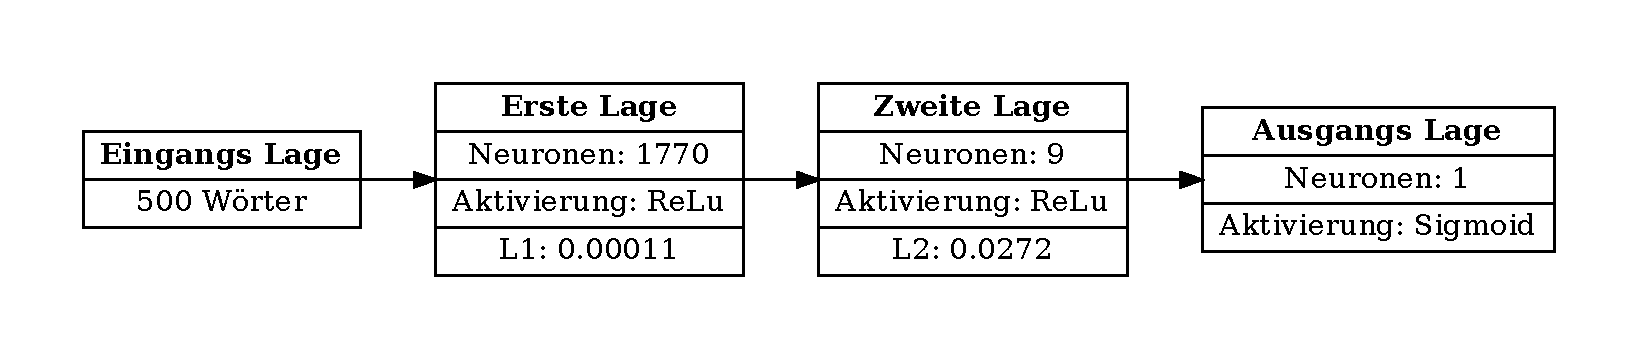
\includegraphics[width=0.8\textwidth]{pictures/modell_scheme.pdf}
    \caption{Schematische Darstellung des mit der \textsc{HYPERAS}-Bibliothek~\cite{hyperas} 
    optimierten DNN.}
    \label{fig:DNN_model}
\end{figure}




